\documentclass[12pt, a4paper]{article}

\usepackage{listings}
\usepackage{color}
\usepackage{enumitem}
\usepackage{amsthm}
\usepackage{amssymb}
\usepackage{listings}
\usepackage{setspace}
\usepackage{graphicx}
\graphicspath{ {./figures/} }


\title{Introduction to Neuroeconomics: How the Brain Makes Decisions}
\author{William Darko}
\date{Summer 2021}

\pagenumbering{arabic}

\begin{document}

\maketitle
\newpage

\tableofcontents

\newpage

\section{About this course}
\paragraph*{}
The intersection of economics, psychology, and neuroscience, form the unified discipline of
Neuroeconomics, with the ultimate goal of creating a single, general theory of human decision making.

Neuroeconomics provides a framework to deeply understand how, and why we make decisions;
neurobiological mecahnisms of decision making, decisions under risk, trust, and coorperation.


\newpage

\section{Resources}

\begin{itemize}
    \item \textbf{Coursera: Intro to Neuroeconomics How the Brain Makes Decisions} 
    taught by professor, and Head of psychology department Vasily Klucharev, at HSE Unviersity 
    (https://www.coursera.org/learn/neuroeconomics)
\end{itemize}

\newpage

\section{Introduction to Neuroeconomics}

\subsection{Origin of Neuroeconomics}

\paragraph*{}
In 2002, Princeton Unvierstiy psychologist Daniel Kahneman PhD, was awarded
the Nobel Memorial Prize for his work in applying psychological insisghts to
economic theory, particularly in areas of judgment, and decision making under 
uncertainty. Vernon L. Smith was also a winner of the award, and also the creator
of the field of experimental economics. Smith established lab experiments as a tool
in empirical economic analysis, especially in the study of alternative market
mechanisms.

\begin{itemize}
    \item \textbf{Paul Glimcher}, the god father of Neuroeconomics.
    \item \textbf{Core Neuroeconomics} or the \textbf{neuroscience of decision making} that studies
    processes connecting sensation and action, by reavealing the neurobiological mechanisms by which
    decisions are made.
    \item \textbf{Extended Neuroeconomics} is a multi-disciplinary field that studies decision making
    by integrating evolutionary, neurobiological, and social science approaches.
    \item \textbf{Optogenetics}: Researchers can modulate activity of targeted neurons using light.
    
    {
        \centering
        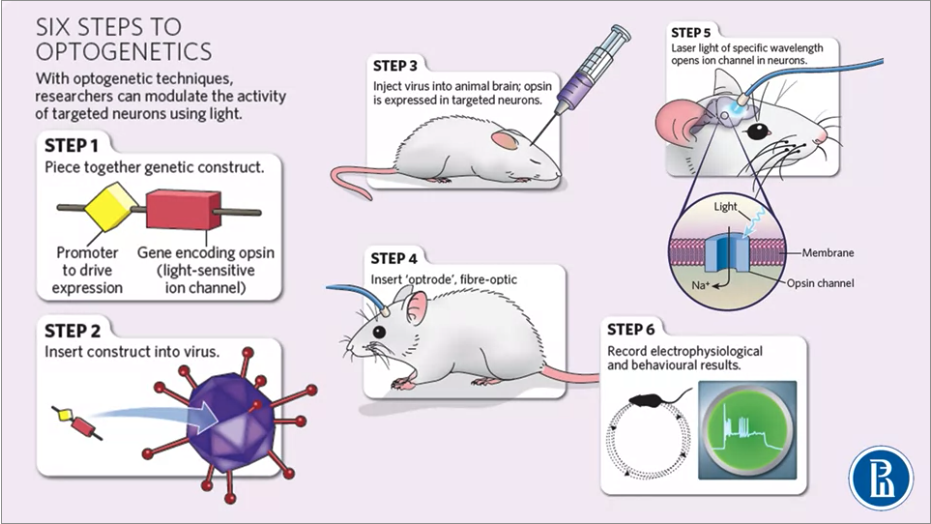
\includegraphics[width=10cm]{optogenetics steps.png}

    }
\end{itemize}

\subsection{Neuroeconomics and Decision-making Theory}

\paragraph*{}

Decision theory is the theory about making decisions... duh.
Examples:
\begin{itemize}
    \item Do I see a red, or green traffic light (sensory system)
    \item Shall I bring the umbrella (depends on knowledge)
    \item A committee must make a decision, but its members have different opinions 
    (How to overcome disagreements)
\end{itemize}

These decisions are based on certain assumptions. The three main assumptions of 
decision theory.
\begin{enumerate}
    \item There are options to choose from.
    \item We choose in a non-random way
    \item Our choices are goal-directed activities/behaviour
\end{enumerate}

\textbf{Ultimately, decision theory is concerned with goal-directed behaviour in the
presence of options}.

\paragraph*{}
Two types of Decision making theory:
\begin{itemize}
    \item \textbf{Normative decision-making theory:} theory about how decisions \textbf{should} be made
    \item \textbf{Descriptive decision-making theory:} theory about how decision are \textbf{actually} made.
\end{itemize}


\end{document}